\chapter{TINJAUAN PUSTAKA}

% Ubah konten-konten berikut sesuai dengan isi dari tinjauan pustaka
\section{Hasil penelitian/perancangan terdahulu}
Dalam penelitian ini, penulis merujuk pada beberapa studi sebelumnya yang relevan. Penelitian-penelitian tersebut memiliki hubungan dengan topik yang sedang diteliti, sehingga dapat digunakan sebagai dasar untuk penelitian ini.

\section{Hasil Penelitian/Perancangan Terdahulu}



\subsection{\emph{Autonomous Thermal Vision Robotic System for Victims Recognition in Search and Rescue Missions}}

Penelitian oleh Cruz Ulloa mengembangkan robot berkaki empat (\emph{quadruped}) menggunakan \emph{Unitree A1} yang dilengkapi dengan kamera termal \emph{Opitris Pi640} dan \emph{Convolutional Neural Network (CNN)} untuk mendeteksi korban dalam misi pencarian di lingkungan pasca-bencana. Penelitian ini berhasil mencapai akurasi lebih dari 90\% dalam kondisi lingkungan sulit, seperti minim cahaya dan puing-puing. Robot ini mampu bergerak secara otonom dan mendeteksi korban dengan cepat di medan yang tidak rata, sehingga dapat membantu tim pencarian dalam menemukan korban yang terperangkap di lokasi bencana\cite{Cruz2021}. Sistem robot dibangun menggunakan \emph{ROS 1 Melodic}. Penelitian ini memiliki kesamaan dengan topik kami yang juga menggunakan \emph{quadruped} dan kamera termal.

\begin{figure} [H] \centering
  % Nama dari file gambar yang diinputkan
  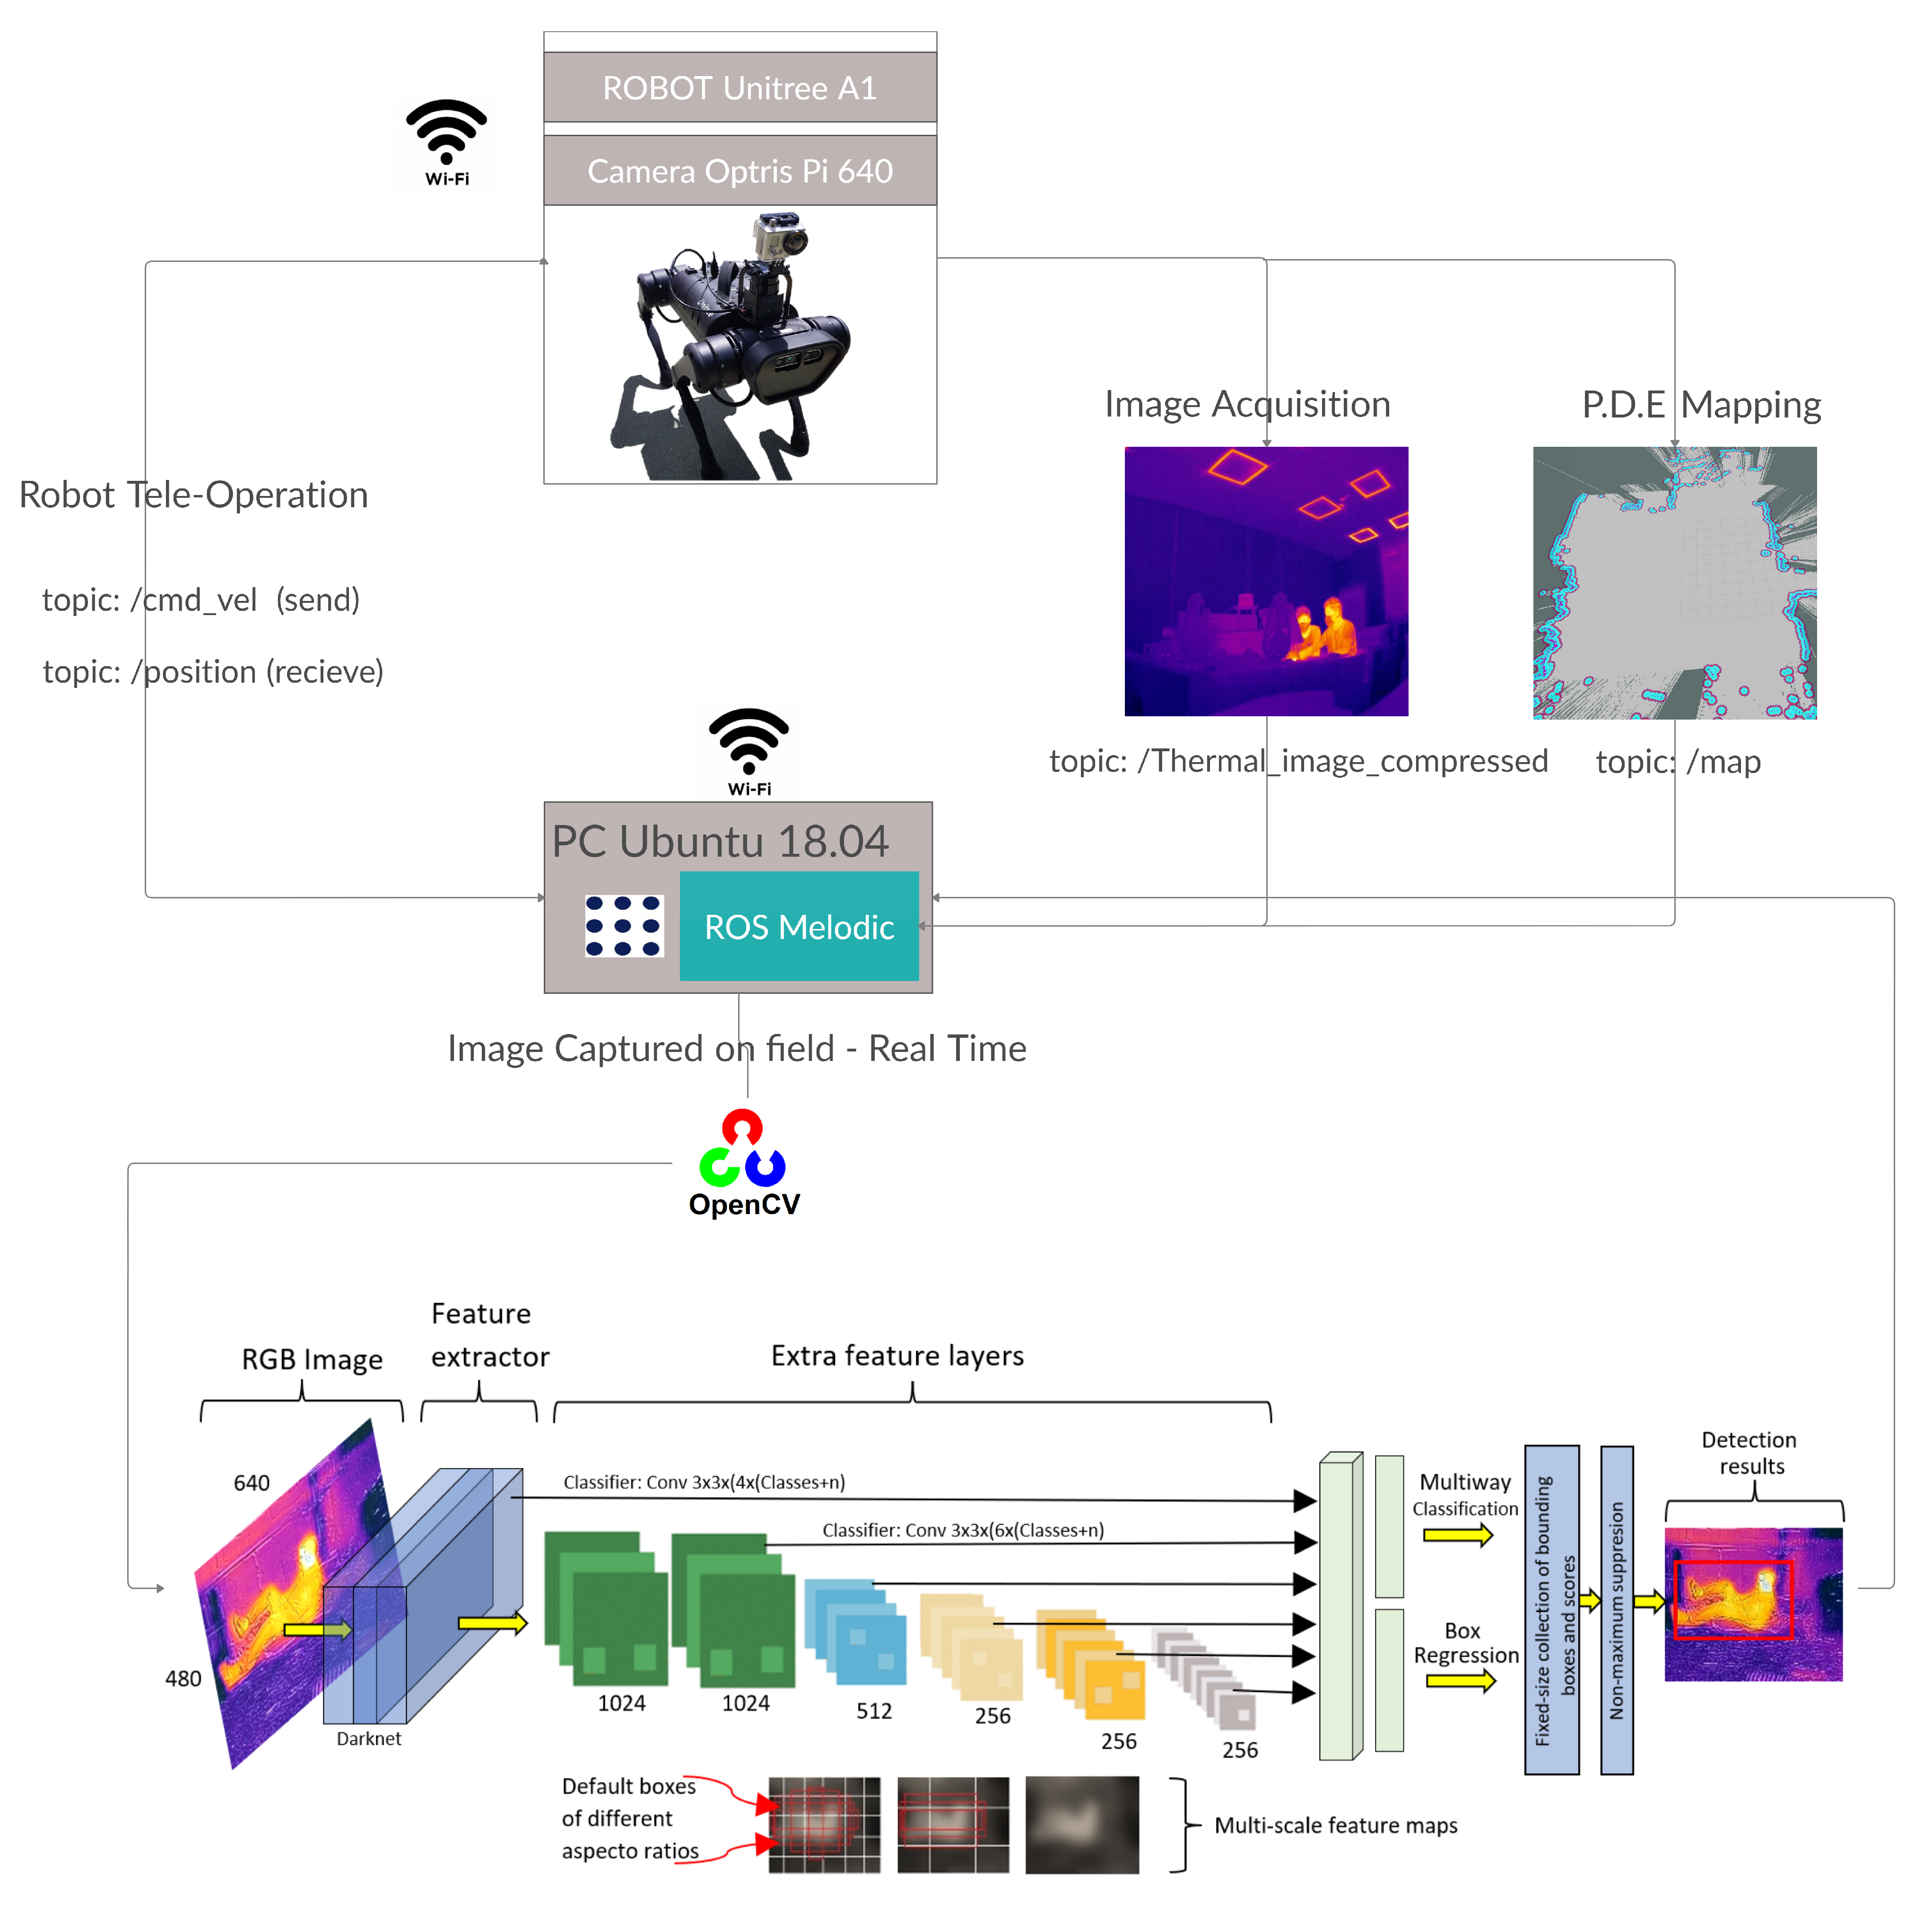
\includegraphics[scale=0.085]{gambar/unitreea1.png}
  % Keterangan gamßbar yang diinputkan
  \caption{\emph{Quadruped robot} dengan kamera termal untuk deteksi korban}
  % Label referensi dari gambar yang diinputkan
  \label{fig:Quadruped  dengan kamera termal untuk deteksi korban}
\end{figure}


\subsection{\emph{Image Processing Technique Applied to Electrical
Substations Based on Drones With Thermal Vision
for Predictive Maintenance}}
Penelitian ini mengusulkan penggunaan \emph{VANT} (Vehículo Aéreo No Tripulado) atau drone, yang dilengkapi dengan dua jenis kamera: \emph{kamera tradisional} untuk menangkap gambar visual dan \emph{kamera termografik} untuk memperoleh gambar inframerah yang dapat menunjukkan suhu komponen di gardu induk. Drone ini dilengkapi dengan sistem navigasi dan pengendalian yang memungkinkan operasi otonom di sekitar gardu induk. Data gambar yang diambil oleh drone diproses menggunakan teknik \emph{image processing} untuk mengidentifikasi \emph{hot spots} atau titik panas pada komponen gardu induk. Hasil analisis ini dapat digunakan untuk memprediksi potensi kerusakan pada komponen dan mengambil tindakan pencegahan yang diperlukan. Penelitian ini menunjukkan bahwa penggunaan drone dengan kamera termal dapat meningkatkan efisiensi dan akurasi dalam pemantauan gardu induk, serta meminimalkan risiko keselamatan bagi petugas yang harus melakukan inspeksi langsung di lokasi gardu \cite{Prieto2022}. Penelitian ini memiliki kesamaan dengan topik kami yang juga menggunakan kamera termal untuk pemantauan komponen gardu listrik.

\begin{figure} [H] \centering
  % Nama dari file gambar yang diinputkan
  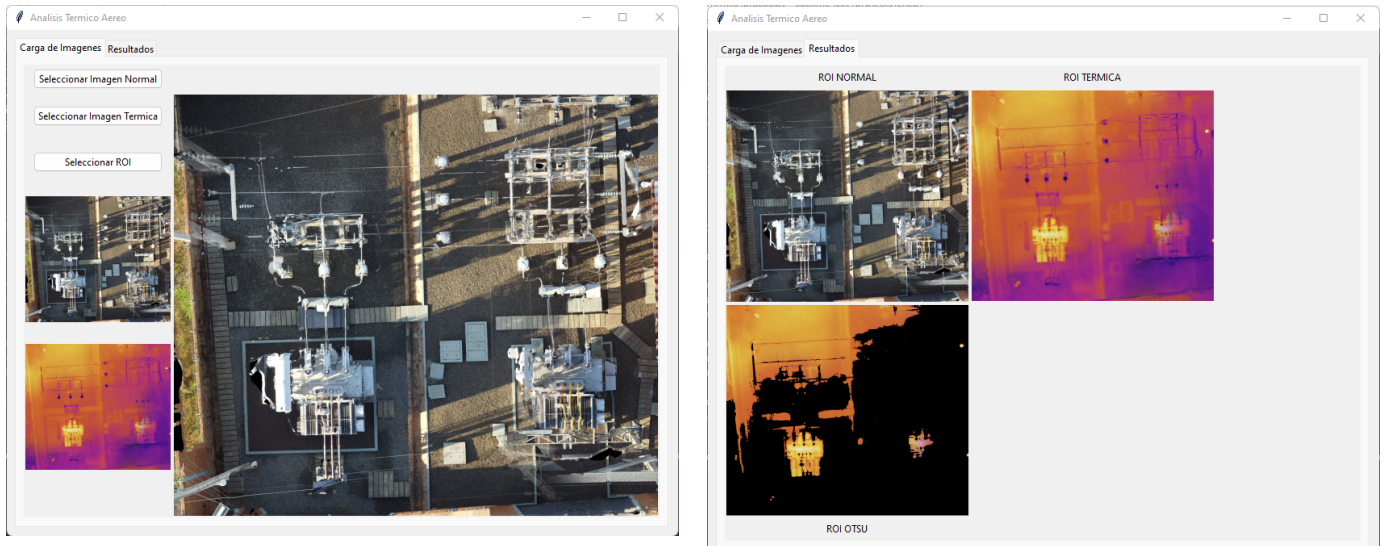
\includegraphics[scale=0.6]{gambar/drone.png}
  % Keterangan gamßbar yang diinputkan
  \caption{Drone dengan kamera termal untuk pemantauan gardu induk}
  % Label referensi dari gambar yang diinputkan
  \label{fig:Drone dengan kamera termal untuk pemantauan gardu induk}
\end{figure}

\subsection{\emph{Direct LiDAR Odometry: Fast Localization With
Dense Point Clouds}}
Penelitian ini berfokus pada pengembangan \emph{Direct LiDAR Odometry} (DLO), sebuah solusi odometri berbasis LiDAR yang \emph{ringan} dan \emph{efisien} untuk robot otonom yang bekerja di lingkungan tanpa sinyal GPS. Sistem ini mengelola informasi peta historis secara efisien dengan cara menyimpan data yang relevan dan mengurangi beban komputasi. DLO memungkinkan penggunaan kembali informasi peta sebelumnya tanpa mengorbankan \emph{kecepatan} dan \emph{akurasi}. DLO menggunakan solver iteratif yang cepat dalam mencocokkan data titik LiDAR, memungkinkan pendaftaran data yang lebih efisien. Teknik ini dipadukan dengan penggunaan kembali struktur data, yang mengurangi waktu pemrosesan dan meningkatkan efisiensi. Sebagai hasilnya, DLO lebih \emph{akurat} dalam menentukan posisi robot dibandingkan dengan metode LiDAR odometry yang ada.

Selain itu, DLO memiliki \emph{beban komputasi yang lebih rendah}, menjadikannya lebih cocok untuk platform robot yang memiliki keterbatasan dalam sumber daya komputasi. Metode ini telah diuji secara ekstensif dalam berbagai lingkungan menantang pada robot udara dan berkaki, termasuk dalam konteks penelitian tim NASA JPL CoSTAR untuk \emph{DARPA Subterranean Challenge} \cite{Chen2022}. Penelitian ini memiliki keterkaitan dengan sistem yang sedang dikembangkan, yang menawarkan sistem lokalisasi tanpa hanya menggunakan GPS, namun tetap \emph{akurat} dan \emph{ringan}. Sistem ini juga diimplementasikan pada robot berkaki (\emph{quadrupped robot}), dengan tujuan untuk memberikan solusi navigasi yang efisien dalam lingkungan yang memiliki medan yang tidak rata dan tidak memiliki sinyal GPS yang memadai.

\begin{figure} [H] \centering
  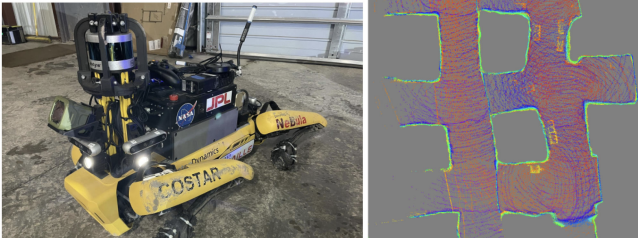
\includegraphics{gambar/dlo.png}
  \caption{Implementasi \emph{DLO} pada \emph{quadruped ledggged robot Boston Dynamics Spot}}
  \label{fig:Implementasi DLO pada quadruped legged robot Boston Dynamics Spot}
\end{figure}

\section{Teori/Konsep Dasar}
Bagian ini berisi pembahasan mengenai teori-teori dasar yang digunakan dalam tugas akhir. Pada bab ini akan dijelaskan mengenai teori-teori yang digunakan dalam penelitian ini. 

\subsection{Gardu listrik}
Gardu listrik merupakan fasilitas yang berfungsi sebagai titik penghubung antara pembangkit listrik dan jaringan distribusi. Gardu berperan penting dalam mengatur dan mendistribusikan tenaga listrik ke konsumen akhir. Terdapat berberapa jenis gardu listrik beberapa diantaranya adalah gardu induk dan gardu pembangkit. Gardu induk adalah fasilitas yang berfungsi untuk mengubah tegangan tinggi menjadi tegangan rendah, sehingga dapat didistribusikan ke konsumen dengan aman. Di sisi lain, gardu pembangkit adalah fasilitas yang terletak di dekat sumber energi, seperti pembangkit listrik tenaga air atau pembangkit listrik tenaga uap, yang berfungsi untuk mengubah energi dari sumber tersebut menjadi energi listrik dan mendistribusikannya ke jaringan listrik. Gardu dilengkapi dengan berbagai peralatan, seperti transformator, pemutus sirkuit, dan isolator, yang berfungsi untuk menjaga kestabilan dan keandalan pasokan listrik. 

\subsubsection{Transformator}
Transformator merupakan komponen esensial dalam sistem kelistrikan, yang berfungsi untuk mengubah tegangan listrik serta memastikan distribusi energi berlangsung secara efisien. Prinsip kerja transformator ini didasarkan pada induksi elektromagnetik, yaitu mengubah tegangan listrik dari tinggi ke rendah atau sebaliknya, sesuai dengan kebutuhan sistem distribusi. Secara umum, transformator gardu induk terdiri dari dua bagian utama, yaitu bagian inti besi dan gulungan kumparan. Bagian inti besi berfungsi sebagai media magnetik yang menghantarkan medan magnet, sedangkan gulungan kumparan berfungsi sebagai media konduktif yang menghantarkan arus listrik. Selain itu, transformator ini juga dilengkapi dengan komponen-komponen penting seperti \emph{bushing}, \emph{tap changer}, dan \emph{cooling system}, yang berperan penting dalam menjaga kinerja serta keandalan transformator. Suhu operasi normal transformator umumnya berkisar antara 40\textdegree{}C hingga 80\textdegree{}C, tergantung pada kapasitas dan spesifikasi teknis transformator tersebut. Namun, ketika suhu melebihi batas aman, biasanya sekitar 105\textdegree{}C hingga 120\textdegree{}C, kondisi tersebut dianggap sebagai \emph{overheating} \cite{tambunan2023kerja}.

\subsubsection{Arester}
\emph{Arester}, atau \emph{lightning arrester}, adalah perangkat yang melindungi sistem kelistrikan dari lonjakan tegangan akibat petir. \emph{Arester} berfungsi untuk mengalihkan arus petir ke tanah, sehingga melindungi peralatan listrik dari kerusakan. Penelitian menunjukkan bahwa untuk memastikan efektivitas \emph{arester}, nilai resistansi pembumian harus rendah, idealnya di bawah 10 $\Omega$. Selain itu, pemeliharaan rutin terhadap \emph{arester} sangat penting untuk memastikan kinerjanya tetap optimal, termasuk pengujian terhadap kondisi lingkungan yang dapat mempengaruhi performanya \cite{Suputra2024}. Suhu operasi \emph{arester} biasanya berkisar antara -40°C hingga 60°C, dan kondisi overheating dapat terjadi jika suhu melebihi batas maksimum yang ditentukan, yang dapat menyebabkan kerusakan permanen pada perangkat tersebut \cite{Kartika2022}.

\subsubsection{Disconnector}
\emph{Disconnector}, atau pemisah, adalah perangkat yang digunakan untuk memutuskan arus listrik dalam sistem distribusi. \emph{Disconnector} berfungsi untuk memisahkan bagian dari sistem kelistrikan untuk keperluan pemeliharaan atau perbaikan tanpa mempengaruhi bagian lain dari jaringan. Pemeliharaan dan pengujian berkala terhadap \emph{disconnector} sangat penting untuk memastikan bahwa perangkat ini berfungsi dengan baik saat dibutuhkan (Henriana & Permata, 2022). Suhu operasi \emph{disconnector} biasanya berada dalam rentang 20°C hingga 40°C, dan overheating dapat terjadi jika suhu melebihi 85°C, yang dapat mengakibatkan kegagalan fungsi (Telaumbanua, 2024).

\subsubsection{Busbar}

\emph{Busbar} adalah komponen penting dalam gardu listrik yang berfungsi sebagai penghubung antara berbagai peralatan listrik. \emph{Busbar} memungkinkan distribusi arus listrik yang efisien dan aman di dalam gardu. \emph{Busbar} biasanya terbuat dari bahan konduktif yang baik, seperti tembaga atau aluminium, dan dirancang untuk menampung arus listrik dalam jumlah besar. Pemeliharaan dan pengujian \emph{busbar} secara rutin diperlukan untuk mencegah kerusakan dan memastikan keandalan sistem distribusi listrik (Telaumbanua, 2024). Suhu operasi \emph{busbar} dapat bervariasi, tetapi umumnya tidak boleh melebihi 90°C untuk mencegah overheating yang dapat merusak isolasi dan struktur busbar itu sendiri (Yang et al., 2016).

\subsubsection{Isolator}

\emph{Isolator} adalah perangkat yang berfungsi untuk memisahkan bagian dari sistem kelistrikan, sehingga mencegah arus listrik mengalir ke bagian yang tidak diinginkan. \emph{Isolator} digunakan untuk menjaga keamanan dan keandalan sistem kelistrikan, terutama saat pemeliharaan dilakukan. \emph{Isolator} dirancang untuk menahan tegangan tinggi dan memiliki karakteristik dielektrik yang baik. Pemeliharaan \emph{isolator} juga penting untuk memastikan bahwa tidak ada kebocoran arus yang dapat menyebabkan kerusakan pada peralatan lainnya. Suhu operasi \emph{isolator} biasanya berkisar antara -30°C hingga 50°C, dan overheating dapat terjadi jika suhu melebihi 70°C, yang dapat mengakibatkan kerusakan pada material isolasi (Moreno, 2017).

\subsubsection{Pemutus Sirkuit (\emph{Circuit Breaker})}

\emph{Pemutus sirkuit} adalah perangkat yang berfungsi untuk melindungi sistem kelistrikan dari arus lebih (\emph{overcurrent}) dan hubung singkat (\emph{short circuit}). \emph{Pemutus sirkuit} dapat secara otomatis memutuskan aliran listrik ketika terdeteksi adanya gangguan, sehingga mencegah kerusakan pada peralatan dan menjaga keselamatan sistem. Terdapat berbagai jenis \emph{pemutus sirkuit}, termasuk \emph{pemutus sirkuit otomatis} (\emph{automatic circuit breaker}) dan \emph{pemutus sirkuit manual} (\emph{manual circuit breaker}), yang masing-masing memiliki aplikasi dan karakteristik yang berbeda. Pemeliharaan dan pengujian berkala terhadap \emph{pemutus sirkuit} sangat penting untuk memastikan bahwa perangkat ini berfungsi dengan baik saat dibutuhkan. Suhu operasi \emph{pemutus sirkuit} biasanya berkisar antara -25°C hingga 55°C, dan overheating dapat terjadi jika suhu melebihi 85°C, yang dapat menyebabkan kerusakan pada mekanisme pemutus (Ilomets et al., 2020).